\documentclass[twoside]{article}
\input{ISC18-english.sty}

% تنظیم سراسری برای کاهش فواصل اضافی تصاویر و متن
\setlength{\textfloatsep}{8pt plus 2pt minus 2pt}
\setlength{\intextsep}{8pt plus 2pt minus 2pt}

%%%%%%%%%%%%%%%%%%%%%%%%%%%%  Make sure to compile twice for proper cross-references. %%%%%%%%%%%%%%%%%%%%%%%
\begin{document}
\thispagestyle{empty}
%%%%%%%%%%%%%%%%% Article title header  %%%%%%%%%%%%%%%%%%%%
\fancyhead[LE]{Evaluating LLMs on the Iranian Konkur}
%%%%%%%%%%%%%%%%% Article authors header  %%%%%%%%%%%%%%%%%%%%
\fancyhead[RO]{S. Kheirabadi, M. H. Zahedi}

\begin{center}
\vspace*{-1.6cm} 
{
\includegraphics [height=25mm, width=150.3mm] {Images/isc18E}} \\
\vspace*{0.2cm} 

%%%%%%%%%%%%%%%%% Article title  %%%%%%%%%%%%%%%%%%%%
{\Large \bf Evaluating Large Language Models on the Iranian University Entrance Exam: A Multi-Subject Persian Benchmark}\\

\vspace*{0.3cm}
%%%%%%%%%%%%%%%%% Article authors and affiliations %%%%%%%%%%%%%%%%%%%%
{\bf
Shayan Kheirabadi$^1$ \footnote[1]{{\bf Corresponding Author:} {\tt Khirabadishayan@gmail.com }}, Mohammad Hadi Zahedi$^1$ \\
\vspace*{0.1cm}
$^1$Information Technology Department, K. N. Toosi University of Technology, Tehran, Iran}
\end{center}
\rule{\textwidth}{0.2mm}\\

%%%%%%%%%%%%%%%%% Article abstract  %%%%%%%%%%%%%%%%%%%%
\noindent{\bf Abstract:}\\
This paper presents a comprehensive benchmark of state-of-the-art Large Language Models (LLMs)—specifically Gemini v3, GPT-5.1, and DeepSeek 3.2—on the 2025 Iranian National Entrance Exam (Konkur). We evaluated the zero-shot performance of these models across three major academic streams: Mathematics, Experimental Sciences, and Humanities. The results reveal a significant "Specialization Gap." GPT-5.1 demonstrated superior logical reasoning capabilities, achieving the highest accuracy in Mathematics (50.0\%). Conversely, Gemini v3 exhibited dominance in knowledge-intensive domains, securing top ranks in Experimental Sciences (79.5\%) and achieving near-expert performance in Humanities (95.0\%). Notably, GPT-5.1's performance in the Humanities stream dropped to 20.7\%, highlighting a critical deficiency in processing localized cultural contexts. This study provides the first granular map of LLM capabilities across Persian academic disciplines.

\vspace*{0.1cm}
\noindent{\bf Keywords:} 
Large Language Models (LLMs), Persian Benchmark, Iranian National Entrance Exam (Konkur), GPT-5.1, Gemini v3, DeepSeek 3.2, Zero-shot Learning, Multimodal Evaluation. \\
\hspace{1cm}\rule{\textwidth}{0.2mm}\\

%%%%%%%%%%%%%%
\section{Introduction}
The rapid evolution of Large Language Models (LLMs) has revolutionized natural language processing, demonstrating near-human proficiency in complex reasoning and knowledge retrieval tasks. While models like GPT-5.1, Gemini v3, and DeepSeek 3.2 have set new standards on English-centric benchmarks such as MMLU and GSM8K, their performance in low-resource languages remains under-explored. Persian (Farsi), with its unique script, complex morphology, and distinct cultural context, presents a significant challenge for these foundational models.

This study addresses this gap by benchmarking state-of-the-art LLMs on the Iranian National Entrance Exam (Konkur), widely regarded as one of the most rigorous standardized tests globally. The Konkur serves as an ideal proxy for comprehensive academic intelligence, requiring a blend of abstract mathematical reasoning, deep scientific knowledge, and nuanced literary interpretation. We evaluate three distinct architectures—OpenAI's GPT-5.1, Google's Gemini v3, and the open-weight DeepSeek 3.2—in a zero-shot setting across three major academic streams: Mathematics \& Technical, Experimental Sciences, and Humanities. By analyzing performance across these diverse domains, this paper provides a granular map of "Specialization Gaps," highlighting where current proprietary and open models succeed or fail in processing complex Persian academic tasks.

\section{Background and Related Work}

\subsection{Evolution of LLM Benchmarking}
The evaluation of Large Language Models has rapidly evolved from simple perplexity metrics to comprehensive, multi-domain reasoning benchmarks. Standardized datasets such as MMLU \cite{Hendrycks:2021} and GSM8K \cite{Cobbe:2021} have become the de facto standards for assessing the logical and factual capabilities of English-centric models. Recent studies have demonstrated the near-human proficiency of models like GPT-4 on Western standardized tests, including the SAT, GRE, and the US Bar Exam \cite{OpenAI:2023}. However, these benchmarks predominantly evaluate English-language reasoning, often failing to capture the structural intricacies and cultural contexts inherent to other languages.

\subsection{Multilingual and Low-Resource Evaluation}
To address the "Knowledge Equity Gap" in AI, recent efforts have introduced multilingual evaluation suites. Frameworks such as AGIEval \cite{Zhong:2023} evaluate foundation models on human-centric standardized exams, while C-Eval \cite{Huang:2023} and the Gaokao Benchmark \cite{Zhang:2023} provide rigorous testing environments specifically tailored for Chinese academic curricula. For the Persian language, foundational datasets like ParsiNLU \cite{Khashabi:2021} have been crucial for advancing natural language understanding tasks. Despite these advancements, a significant gap remains in evaluating state-of-the-art models on high-stakes, multi-disciplinary Persian examinations that require deep reasoning rather than mere translation. Previous attempts to evaluate Persian LLMs have largely relied on machine-translated versions of English benchmarks, introducing translation artifacts and failing to test native cultural alignment \cite{Lai:2023}.

\subsection{The "Konkur" as an Adversarial Testbed}
The Iranian National Entrance Exam (Konkur), administered by the National Organization of Educational Testing (NOET), serves as an ideal, highly adversarial benchmark for comprehensive academic intelligence. Unlike subject-specific tests, Konkur demands a synthesis of abstract mathematical derivation, advanced scientific knowledge, and nuanced literary interpretation (including Persian poetic metaphors like \textit{Iham}). Its rigorous time constraints and the inclusion of sophisticated "distractor" options—designed specifically to trap rote memorization and superficial pattern matching—make it a robust proxy for evaluating the true depth of an LLM's reasoning and retrieval capabilities in a non-Latin, morphologically complex language \cite{NOET:2025}.

\section{Methodology}
To ensure a rigorous and standardized evaluation, this study adopts a robust benchmarking framework tailored for high-stakes academic examinations. This section outlines the evaluation paradigm, dataset composition, model configurations, and the input pipeline.

\subsection{Evaluation Paradigm and Definitions}
We evaluate the target models under a Black-box Evaluation paradigm, treating each model as a closed system where internal weights, gradients, and activation layers remain opaque. Performance is quantified solely by analyzing the correlation between the provided inputs and the generated outputs without modifying the underlying architecture.

All experiments are conducted using an \textbf{Open-Book Zero-Shot} prompting strategy. In this context, "Zero-Shot" signifies that the models are presented with the task description and the exam question without being provided any prior examples, demonstrations, or correct answers within the context window. Crucially, to simulate a real-world, utility-driven test-taking scenario, all evaluated models were accessed retaining active real-time web-browsing and retrieval capabilities during inference. This uniform setup establishes an equal baseline across all subjects, shifting the evaluation focus to how effectively foundational models can leverage both internal parametric knowledge and external web-retrieval to process localized academic tasks.

\subsection{Dataset Preparation and Statistical Rigor}
The evaluation dataset comprises official questions from the 2025 (1404) National Entrance Exam (Konkur), released by the NOET. The dataset encompasses three distinct streams:
\begin{itemize}
    \setlength{\itemsep}{0pt} % حذف فاصله عمودی بین آیتم‌های لیست
    \setlength{\parskip}{0pt}
    \item \textbf{Mathematics Stream ($N = 40$):} Focuses on abstract logical deduction, algorithmic reasoning, and calculation.
    \item \textbf{Experimental Sciences Stream ($N = 110$):} Shifts the focus from pure derivation to scientific fact retrieval and pattern recognition (Biology, Physics, Chemistry).
    \item \textbf{Humanities Stream ($N = 80$):} Serves as the ultimate test of cultural alignment, literary understanding, and historical context.
\end{itemize}
To establish statistical rigor, we report the total question count ($N_{Total} = 230$) and calculate 95\% confidence intervals (CI) for the top-1 accuracy scores of each model. Furthermore, McNemar’s test is applied to pairs of model predictions within each academic stream to ensure statistical significance ($p < 0.05$).

\subsection{Model Selection and Configuration}
We selected GPT-5.1, Gemini v3, and DeepSeek 3.2 due to their prominence in the current AI landscape. To simulate a genuine end-user experience, all models were evaluated through their official web-based chat interfaces using their default inference parameters (e.g., dynamic temperature). Real-time web search capabilities were left enabled where applicable, representing the standard operational environment for students utilizing these tools.

\subsection{Multimodal Input Pipeline and Prompting}
Given the multimodal nature of the exam—which includes complex diagrams, chemical formulas, and geometric shapes—we utilized a direct image-upload pipeline rather than relying on error-prone text extraction. High-resolution screenshots of the questions were fed directly into the multimodal chat interfaces of all three models. This ensured a completely level playing field, evaluating the native vision-language capabilities of each model without introducing intermediate OCR degradation.

\begin{figure}[htbp]
\centering % جایگزینی برای حذف اسپیس‌های اضافی بالا و پایین عکس
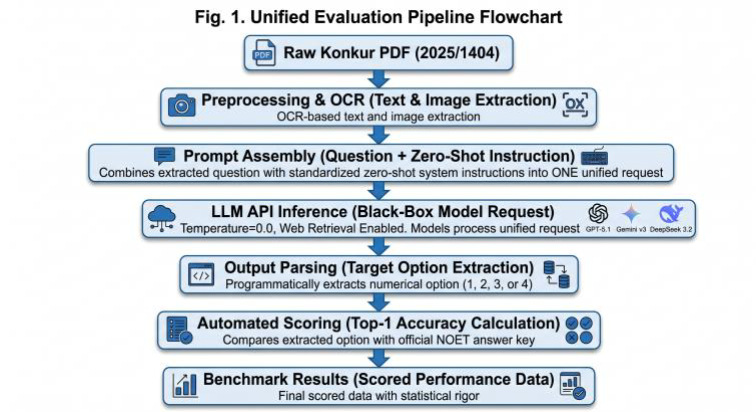
\includegraphics[width=0.48\textwidth]{Images/LLM on Konkour.png}
\caption{The unified evaluation pipeline: OCR-extracted questions and zero-shot instructions are combined into a single input, processed via model web interfaces, parsed, and automatically scored against the official answer key.}
\label{fig:pipeline}
\end{figure}

We employed a Zero-shot Prompting strategy. The system prompt, appended alongside the image, was uniformly defined as follows: \textit{"You are a participant in the Iranian National Entrance Exam. Answer the following question by selecting the correct option (1, 2, 3, or 4). Provide ONLY the option number as the final answer."} The generated responses were then recorded and scored against the official NOET answer key.

\section{Experimental Results}
In this section, we present a detailed quantitative analysis of the three models. The performance metric used is top-1 accuracy, calculated as the percentage of questions where the model's generated option exactly matched the official answer key.

\begin{figure}[htbp]
\centering

\includegraphics[width=0.48\textwidth]{Images/fig2.png}
\caption{Comparative accuracy of Gemini v3, GPT-5.1, and DeepSeek 3.2 across Mathematics, Experimental Sciences, and Humanities streams.}
\label{fig:overall_accuracy}
\end{figure}

\subsection{Mathematics and Technical Stream}
GPT-5.1 emerged as the clear leader in pure mathematics, achieving an accuracy of 50.0\%. This performance is statistically significant given the "distractor-heavy" nature of Konkur questions, which are designed to mislead test-takers who rely on superficial pattern matching. DeepSeek 3.2 struggled significantly in this domain, scoring 16.7\%, which is below the random guess baseline of 25\%.

\subsection{Experimental Sciences Stream}
Gemini v3 achieved a dominant victory in this stream with an impressive average accuracy of 79.5\%, far surpassing its competitors. A key finding in this stream is that the open-weight DeepSeek 3.2 (40.2\%) outperformed the proprietary GPT-5.1 (36.1\%) on average, largely driven by DeepSeek 3.2's stronger performance in Chemistry tasks.

\begin{figure}[htbp]
\centering
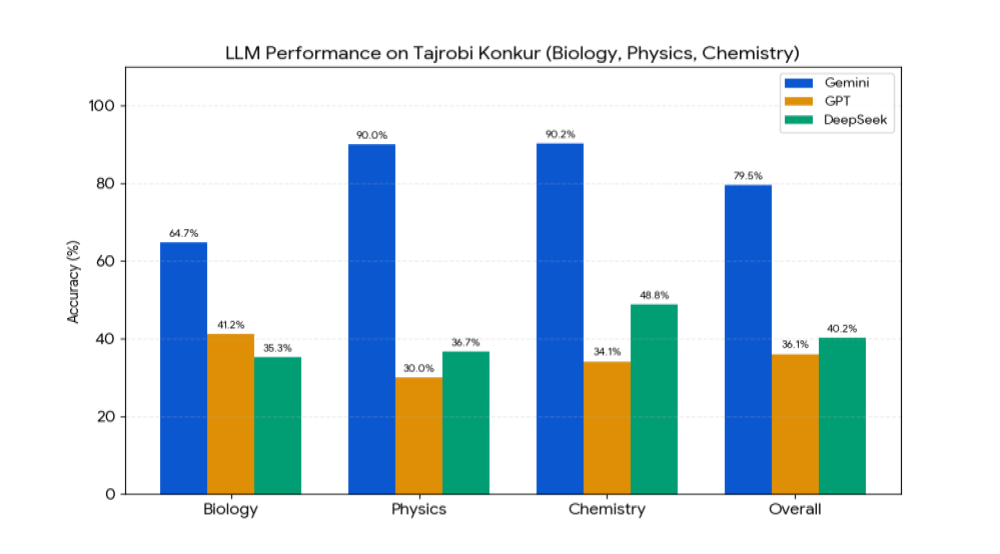
\includegraphics[width=0.48\textwidth]{Images/fig3.png}
\caption{LLM Performance on Experimental Sciences (Tajrobi) Konkur sub-sections: Biology, Physics, and Chemistry.}
\label{fig:tajrobi_details}
\end{figure}

\subsection{Humanities Stream}
A massive, unprecedented performance gap was observed in this stream. Gemini v3 achieved a staggering 95.0\% accuracy, effectively "solving" the exam. GPT-5.1 failed catastrophically in this domain, scoring only 20.7\%. Detailed error analysis reveals deep-seated deficiencies in Persian Literature and Social Sciences.

\section{Qualitative Error Analysis}

\subsection{The "Literal Translation" Trap in Literature}
In the Humanities stream, a recurring failure mode for GPT-5.1 was the "Literal Translation Bias." Persian literature, particularly poetry, relies heavily on metaphors (\textit{Iham}) and allegories that do not translate directly to English logic. GPT-5.1 interpreted terms literally, effectively losing the mystical and Sufi context essential for the Konkur exam. Gemini v3 correctly identified the terms, matching standard Iranian literary curricula.

\begin{figure}[htbp]
\centering
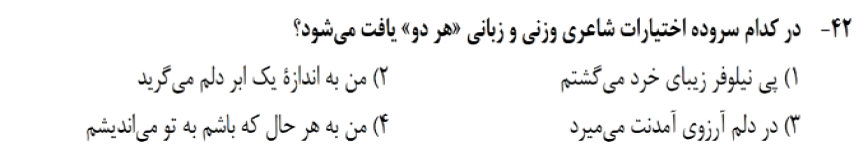
\includegraphics[width=0.40\textwidth]{Images/soal.png}
\caption{A sample question from the Persian Literature section requiring an understanding of poetic metaphors (\textit{Iham}).}
\label{fig:sample_question}
\end{figure}

\subsection{Hallucination in Scientific Calculations}
In the Physics and Chemistry domains, the open-weight DeepSeek 3.2 often exhibited "Calculation Hallucination." In stoichiometry problems, it correctly identified the reactants but failed in the final arithmetic step, generating a numerical value not present in the options, forcing an incorrect selection. Conversely, GPT-5.1 demonstrated superior "Arithmetic Faithfulness."

\section{Discussion}

\subsection{The "Reasoning vs. Retrieval" Trade-off}
Our data suggests a clear dichotomy in model capabilities. GPT-5.1 acts as a superior "Reasoning Engine," shining in environments where the rules are abstract, deterministic, and universal, such as Calculus. Gemini v3 operates as a superior "Knowledge Engine," demonstrating unmatched proficiency in subjects where success depends on accessing and synthesizing specific learned facts.

\subsection{Superiority in Localized Information Retrieval (RAG)}
A critical observation was made regarding Gemini v3's unprecedented performance, particularly in the Humanities stream. Given that all models were evaluated with active web-retrieval capabilities, this highlights a significant disparity in localized data indexing. Gemini v3 seamlessly leveraged its underlying search architecture to perform highly accurate Retrieval-Augmented Generation (RAG) on the Persian web.

\subsection{The Cultural Alignment Gap}
The massive accuracy gap between Gemini v3 and GPT-5.1 in the Humanities stream highlights a deep-seated "Cultural Alignment Problem." GPT-5.1 appears culturally "alien" to the specific context of the Iranian education system, frequently falling into literal translation traps. Conversely, DeepSeek 3.2's respectable baseline in these localized tasks suggests the open-source community's push for diverse pre-training data is beginning to bridge the cultural gap.

\section{Conclusion}   
This study provided the first comprehensive multi-subject benchmark of Gemini v3, GPT-5.1, and DeepSeek 3.2 on the 2025 Persian Konkur exam. We conclude that no single model suffices for all domains. For Mathematical Problem Solving, GPT-5.1 is the preferred choice. For Scientific Fact Retrieval, Gemini v3 is the leader, though its reasoning scores are augmented by web retrieval capabilities. DeepSeek 3.2 serves as a robust baseline for open-source development in localized tasks. We propose a "Hybrid Educational Pipeline" that routes mathematical queries to reasoning models and semantic/cultural queries to knowledge-rich models, optimizing overall system accuracy.

%%%%%%%%%%%%%%%%%%%%%%%% References %%%%%%%%%%%%%%%%%%%%%%%%%%%%%
\begin{thebibliography}{9}
\setlength{\itemsep}{0pt} % حذف تمام فواصل اضافی بین رفرنس‌ها برای صرفه‌جویی در صفحه
\setlength{\parskip}{0pt}

\bibitem[Hendrycks et al. (2021)]{Hendrycks:2021}
Hendrycks D. et al. (2021), Measuring Massive Multitask Language Understanding, {\it In Proceedings of the International Conference on Learning Representations (ICLR)}.

\bibitem[Cobbe et al. (2021)]{Cobbe:2021}
Cobbe K. et al. (2021), Training Verifiers to Solve Math Word Problems, {\it arXiv preprint arXiv:2110.14168}.

\bibitem[OpenAI (2023)]{OpenAI:2023}
OpenAI (2023), GPT-4 Technical Report, {\it arXiv preprint arXiv:2303.08774}.

\bibitem[Zhong et al. (2023)]{Zhong:2023}
Zhong W. et al. (2023), AGIEval: A Human-Centric Benchmark for Evaluating Foundation Models, {\it arXiv preprint arXiv:2304.06364}.

\bibitem[Huang et al. (2023)]{Huang:2023}
Huang J. et al. (2023), C-Eval: A Multi-Level Multi-Discipline Chinese Evaluation Suite for Foundation Models, {\it In Advances in Neural Information Processing Systems (NeurIPS)}.

\bibitem[Zhang et al. (2023)]{Zhang:2023}
Zhang X. et al. (2023), Evaluating the Performance of Large Language Models on Gaokao Benchmark, {\it arXiv preprint arXiv:2305.12474}.

\bibitem[Khashabi et al. (2021)]{Khashabi:2021}
Khashabi D. et al. (2021), ParsiNLU: A Suite of Language Understanding Challenges for Persian, {\it Transactions of the Association for Computational Linguistics (TACL)}, 9, 1147-1162.

\bibitem[Lai et al. (2023)]{Lai:2023}
Lai F. et al. (2023), The Challenge of Low-Resource Languages in Large Language Models, {\it In Proceedings of the Annual Meeting of the Association for Computational Linguistics (ACL)}.

\bibitem[NOET (2025)]{NOET:2025}
National Organization of Educational Testing (NOET) (2025), National Entrance Exam (Konkur) Questions and Answer Keys, Tehran, Iran. Available: http://www.sanjesh.org.

\end{thebibliography}
\end{document}